\subsection{Code Smells}
\label{smells}
Using the methodology described in section~\ref{smells:methodology}, we sampled 10 best practices in javascript from AirBNB javascript coding style guide~\cite{airbnb_code} and compared Copilot syggestions when prompted with a input method(shown in section~\ref{smells:input}) and evaluated using methodology shown in section~\ref{smells:evaluation}. 

Copilot suggested the best practice from the coding guide for only one out of the ten coding standards we tested, i.e, 1 out of 10 instances Copilot had the recommended way as its top suggestion. Moreover, only 2 out of remaining 9 standards had the best practice in Copilot top 10 suggestions currently viewable. Copilot did not have the best practice in any of its top 10 suggestions for 7 standards out of 10 coding standards we tested.

% Copilot performed significantly worse than the Pythonic Idioms we showed in Section~\ref{secidioms}, As Copilot is closed source, we cannot find the reason behind this but one could argue that lack of data for JavaScript compared to python could be a reason for this behaviour. 

Table~\ref{tab:all_bp} shows the complete list of all the coding standards we tested on Copilot sampled from the AirBNB Coding Style guide~\cite{airbnb_code} and the ranking of the best practice in Copilot suggestions (if it exists).

\begin{table}[ht]
    \centering
    \begin{tabular}{|L|c|}
    \hline
         \textbf{Best Practice  Title} & \textbf{Copilot Suggestion Matched?} \\
         & (out of 10 suggestions) \\
         \hline
         Usage of Object method shorthand & No \\
         \hline
         Array Creating Constructor & 6\textsuperscript{th} \\
         \hline
         Copying Array Contents  & No \\
         \hline
         Logging a Function &  No \\
         \hline
         Exporting a Function & No \\
         \hline
         Sum of Numbers & 9\textsuperscript{th} \\
         \hline
         Accessing Properties & 1\textsuperscript{th} \\
         \hline
         Switch case usage & No \\
         \hline
         Return value from Function with a condition check & No \\
         \hline
         Converting Array-like object to an Array  & No \\
         \hline
    \end{tabular}
    \caption{List of all JavaScript Best Practices tested on Copilot.}
    \label{tab:all_bp}
\end{table}

Figure~\ref{fig:bp_1} shows the Best Practice for Copying Array Contents, showing user input (i.e., Human Input), the top suggestion by Copilot and the recommended way suggested by AirBNB JavaScript coding style guide~\cite{airbnb_code}.

\begin{figure}[hbt!]
    \centering
    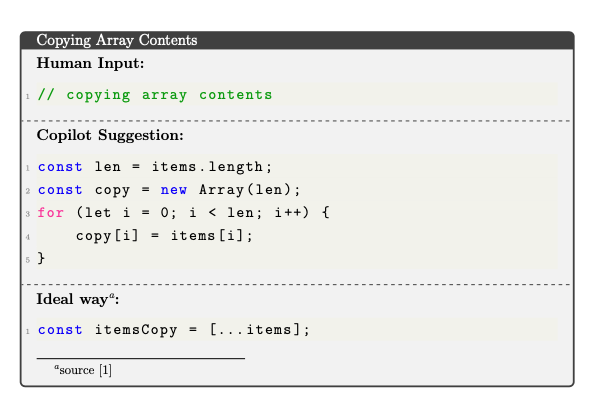
\includegraphics[width=\linewidth]{Figures/bp_1.png}
    \caption{Best Practice for Copying Array Contents and Copilot Suggestion.}
    \label{fig:bp_1}
\end{figure}

The results show that Copilot performed worse than the language idioms~(shown in chapter~\ref{chapter:idioms}). Copilot did not suggest the best practice as its first suggestion for 7 out of 10 coding standards we tested. This shows that current AI-supported
code completion tools like Copilot cannot suggest coding standards in its suggestions even though the coding standards are the sampled from widely accepted coding style guide.

All the Best Practices shown in Table~\ref{tab:all_bp} can be found in the \repl{} including the code used as input (i.e., human input), the top suggestion by Copilot and the best practice from AirBNB JavaScript coding style guide~\cite{airbnb_code}.

There could be many reasons for this performance like the public repositories do not always follow coding standards, Copilot cannot detect coding style from repositories that have contribution guides including the coding standards followed in the project. 
Copilot being closed source we cannot investigate the potential reasons behind this behavior and recommend ways to fix this issue improving the performance of Copilot.

We did not test Copilot for suggesting project specific coding styles because Copilot does not have the feature to customise its suggestions based on preferences~\cite{Copilot-web}.
However, \cct{} like Copilot should follow coding style guides and adapt their code suggestions to match the coding style used in the project. 
For example, if a user is working on a project where one of the coding style guideline says to leave a blank line after blocks and before the next statement~\cite{airbnb_code}. As a productivity tool, the ideal behaviour for \cct{} like Copilot is to detect the coding style guideline from existing code in the project and always suggest code that follows the guideline. 

% \begin{tcolorbox}[title=Copying Array Contents,boxsep=.15mm]
%     %https://tex.stackexchange.com/questions/337909/tcolorbox-tcbline-style
% \textbf{Human Input:}
% \begin{lstlisting}[language=JavaScript]
% // copying array contents
% \end{lstlisting}
% \tcbline
% \textbf{Copilot Suggestion:}
% \begin{lstlisting}[language=JavaScript]
% const len = items.length;
% const copy = new Array(len);
% for (let i = 0; i < len; i++) {
% 	  copy[i] = items[i];
% }
% \end{lstlisting}
% \tcbline
% \textbf{Ideal way\footnote{source \cite{airbnb_code}}:}
% \begin{lstlisting}[language=JavaScript]
% const itemsCopy = [...items];
% \end{lstlisting}
% \end{tcolorbox}

%%%%%% TODO: remember to update the screenshot if the source citation is different from the citation in the text %%%%%%

